\documentclass{article}
\usepackage{amsmath,amsthm}
\usepackage{amssymb,latexsym}
\usepackage{float}
\usepackage{fullpage}
\usepackage{times}

% graphs
\usepackage{tikz}
\usepackage[edges,linguistics]{forest}
\usetikzlibrary{automata,positioning,shadows,arrows.meta}

\tikzset{initial text={}}

% grammars
\usepackage{listings}

\lstset{
  basicstyle=\itshape,
  xleftmargin=3em,
  literate={->}{$\rightarrow$}{2}
           {epsilon}{$\epsilon$}{1}
}

\newtheorem{theorem}{Theorem}
\newtheorem{corollary}[theorem]{Corollary}
\newtheorem{question}[theorem]{Question}
\newtheorem{lemma}[theorem]{Lemma}
\newtheorem{observation}[theorem]{Observation}
\newtheorem{proposition}{Proposition}
\newtheorem{definition}[theorem]{Definition}
\newtheorem{claim}[theorem]{Claim}
\newtheorem{fact}[theorem]{Fact}
\newtheorem{assumption}[theorem]{Assumption}
\newtheorem{example}{Example}
\newtheorem{conjecture}[theorem]{Conjecture}
\newtheorem{alg}[theorem]{Algorithm}

\newcommand{\set}[1]{{\left\{#1\right\}}}    % braces for set notation
\newcommand{\ve}[1]{\mathbf{#1}}
\newcommand{\abs}[1]{\left\lvert #1 \right\rvert}
\newcommand{\poly}{\operatorname{poly}}
\newcommand{\complex}{{\mathbb C}}
\newcommand{\reals}{{\mathbb R}}
\newcommand{\ints}{{\mathbb Z}}
\newcommand{\nats}{{\mathbb N}}
\newcommand{\proj}[1]{\mbox{$|#1\rangle \!\langle #1 |$}}
\newcommand{\enc}[1]{\left<#1\right>}
\newcommand{\spa}[1]{\mathcal{#1}}
\newcommand{\ayes}{A_{\rm yes}}
\newcommand{\ano}{A_{\rm no}}

\begin{document}

\title{
    CMSC 303 Introduction to Theory of Computation, VCU\\
    Assignment: 4\\
    Name: Steven Hernandez
}

\date{}

\maketitle
\vspace{-10mm}

Note: question 2.a uses http://www.cs.ucsb.edu/~cappello/136/lectures/17cfls/slides.pdf as a resource.

\begin{enumerate}
    \item % 1
        \begin{enumerate}
            \item
                \begin{forest}
                    [E
                        [T
                            [F
                                [2]
                            ]
                        ]
                    ]
                \end{forest}
            \item
                \begin{forest}
                    where n children=0{
                       tier=word,
                    }{
                       inner xsep=0pt,
                    },
                    for tree={
                       if n children=0{
                           font=\itshape,
                           tier=terminal,
                       }{},
                       fit=band,
                    },
                    forked edges,
                    [E
                        [E
                            [E
                                [T
                                    [F
                                        [2]
                                    ]
                                ]
                            ]
                            [+]
                            [T
                                [F
                                    [2]
                                ]
                            ]
                        ]
                        [+]
                        [T
                            [F
                                [2]
                            ]
                        ]
                    ]
                \end{forest}
            \item
                \begin{forest}
                    where n children=0{
                       tier=word,
                    }{
                       inner xsep=0pt,
                    },
                    for tree={
                       if n children=0{
                           font=\itshape,
                           tier=terminal,
                       }{},
                       fit=band,
                    },
                    forked edges,
                    [E
                        [T
                            [T
                                [F
                                    [(]
                                    [E
                                        [E
                                            [T
                                                [F
                                                    [2]
                                                ]
                                            ]
                                        ]
                                        [+]
                                        [T
                                            [F
                                                [2]
                                            ]
                                        ]
                                    ]
                                    [)]
                                ]
                            ]
                            [\textit{$\times$}]
                            [F
                                [(]
                                [E
                                    [T
                                        [F
                                            [2]
                                        ]
                                    ]
                                ]
                                [)]
                            ]
                        ]
                    ]
                \end{forest}
        \end{enumerate}
    \item % 2
        \begin{enumerate}
            \item
                Using languages $A = \set{a^mb^nc^n | m,n \ge 0}$ and $B = \set{a^nb^nc^m | m,n \ge 0}$, so the class of context-free languages are not closed under intersection.

                Suppose the opposite, that context-free languages are in fact closed under intersection.
                This would imply that $A \cap B$ must be a context-free language.
                But what would this mean?

                This new language could be written $C = A \cap B = \set{a^nb^nc^n | m,n \ge 0}$.
                Notice we now have 3 sections which each must be of the same size.
                The previous languages $A$ and $B$ were easily handled by the stack approach of a PDA.
                For $B$, simply place each symbol of $a^n$ into the stack.
                For $b$, as each symbol is read from the input, simply pop off an equal number of symbols from the stack.
                This is similar for $A$.

                Notice however, both $A$ and $B$ only need to compare the length of two sections.
                The third section does not matter.

                Because a PDA only has one stack, as we read each letter for $b$ in $C$ (after having read in all $a$ to the stack) we are throwing the letter away and popping $a$ from the stack.
                After handling both $a$ and $b$, we no longer have any way of knowing the size of $n$ because the stack no longer contains that information.
                Thus $C$ is not a context-free language and as such context-free languages are not closed under intersection.
            \item
                Show the set of context-free languages are not closed under complement.

                Proof: We use DeMorgan's law: $\overline{(A \cup B)} = \overline{A} \cap \overline{B}$ which can be rewritten: $(A \cap B) = \overline{\overline{A} \cup \overline{B}}$ where $A$ and $B$ are context-free languages.

                Assume the complement of a context-free language is also a context-free grammar. Then using DeMorgan's Law above, we see this implies that the intersection of two context-free languages $A \cap B$ is closed, which we showed is not true in question 2.a. Thus, contradiction.
        \end{enumerate}
    \item % 3
        \begin{enumerate}
            \item
                \begin{lstlisting}
                    S -> 0 | 1 | 0T0 | 1T1
                    T -> epsilon | 1T | 0T
                \end{lstlisting}

                Trivially $0$ and $1$ match.
                $0T0$ $1T1$ ensure that the first and last symbol are the same before moving past $S$ into $T$.
                $T$ simply allows you to add any symbols $\in \Sigma_{epsilon}$ recursively within the string obtained above.
            \item
                \begin{lstlisting}
                    S_0 -> 0 | 1 | 0S_{odd} | 1S_{odd}
                    S_{odd} -> epsilon | 0S_{even} | 1S_{even}
                    S_{even} -> 0 | 1 | 0S_{odd} | 1S_{odd}
                \end{lstlisting}

                Think of the labels such that $S_{odd}$ means we have an odd length currently, thus we can only add $epsilon$ of one symbol, which then means we now have an even number of symbols (thus the $S_{even}$).
            \item
                \begin{lstlisting}
                    S -> epsilon | 0 | 1 | 0S0 | 1S1
                \end{lstlisting}

                Unlike $a$, the only variable is $S$, this is because each time we recurse, we want to ensure whatever the sub-string contains, it always begins and ends with the same symbol, thus maintaining the palindrome.
            \item
                \begin{lstlisting}
                    S -> S
                \end{lstlisting}

                The grammar continues recursively forever.
                Never reaching only terminals, thus never reaching an accept state.
            \item
                \begin{lstlisting}
                    S ->   X$C$X | C$X | X$C | C
                    C ->   1C1 | 0C0 | $ | $X$
                    X ->   $X | 1X | 0X | epsilon
                \end{lstlisting}

                The idea for this grammar is that $C$ always builds a palindrome.
                Note how from $C$, we either recursively wrap $C$ with $0$ or $1$.
                After which, we can leave $\$$ in the center.

                From the first step, if there are any symbols to the left or right of $C$, we delimite it with a $\$$.
                This keeps the grammar matching the language.

                This produces the language when $i = n$ and $j = n+1$, however does not account for $i = n$ and $j = n + t$ where $t > 1$.
                So, notice $C \rightarrow \$X\$$.
                This allows the palindrome we were building to have non-palindrome-like items in the middle of this palindrome.
                Notice though, that these symbols are delimited by $\$$ so that we keep separate the palindrome from earlier.
        \end{enumerate}
    \item % 4
        \begin{enumerate}
            \item
                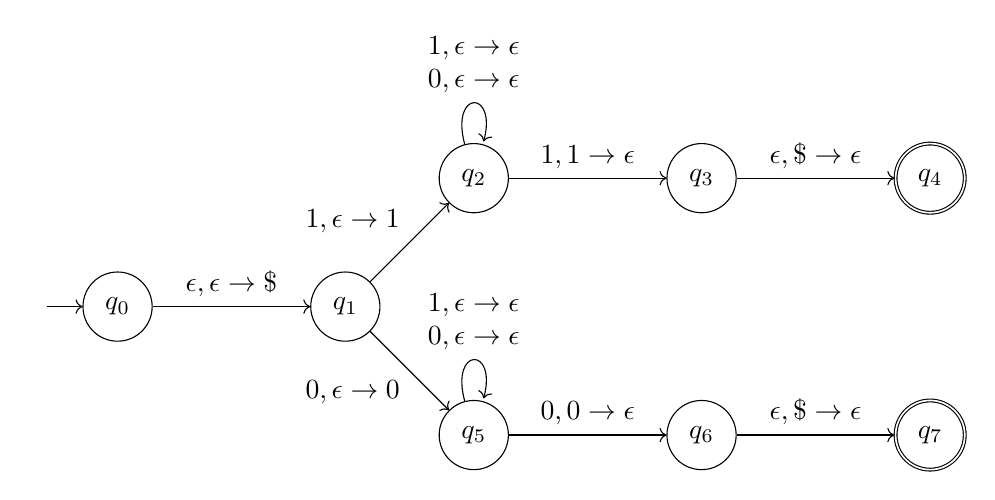
\begin{tikzpicture}
                   \node[state,initial] (q_0)   {$q_0$};
                   \node[state] (q_1) [right=2cm of q_0] {$q_1$};
                   \node[state] (q_2) [above right=of q_1] {$q_2$};
                   \node[state] (q_3) [right=2cm of q_2] {$q_3$};
                   \node[state,accepting] (q_4) [right=2cm of q_3] {$q_4$};
                   \node[state] (q_5) [below right=of q_1] {$q_5$};
                   \node[state] (q_6) [right=2cm of q_5] {$q_6$};
                   \node[state,accepting] (q_7) [right=2cm of q_6] {$q_7$};
                    \path[->]
                    (q_0) edge [above] node {$\epsilon,\epsilon\rightarrow\$$} (q_1)
                    (q_1) edge [above left] node {$1,\epsilon\rightarrow1$} (q_2)
                          edge [below left] node {$0,\epsilon\rightarrow0$} (q_5)
                    (q_2) edge [above] node {$1,1\rightarrow\epsilon$} (q_3)
                          edge [loop above,align=left] node {$1,\epsilon\rightarrow\epsilon$ \\ $0,\epsilon\rightarrow\epsilon$} (q_2)
                    (q_3) edge [above] node {$\epsilon,\$\rightarrow\epsilon$} (q_4)
                    (q_5) edge [above] node {$0,0\rightarrow\epsilon$} (q_6)
                          edge [loop above,align=left] node {$1,\epsilon\rightarrow\epsilon$ \\ $0,\epsilon\rightarrow\epsilon$} (q_5)
                    (q_6) edge [above] node {$\epsilon,\$\rightarrow\epsilon$} (q_7)
                    ;
                \end{tikzpicture}

                Notice however, this solution does not require a stack.
                The language could be modeled easily by an NFA with two branches as seen above.

                Instead, a PDA where the stack is required, can be modeled as such:

                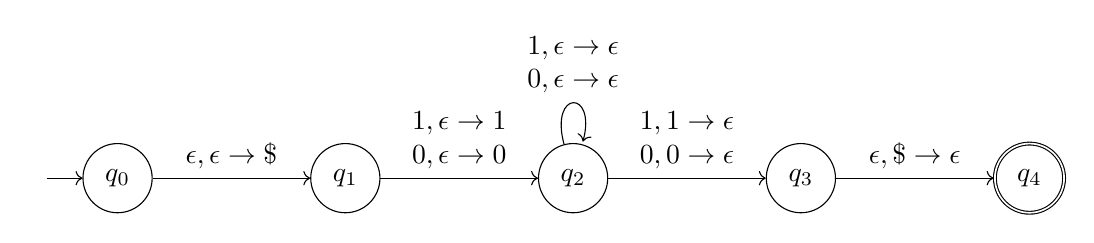
\begin{tikzpicture}
                   \node[state,initial] (q_0)   {$q_0$};
                   \node[state] (q_1) [right=2cm of q_0] {$q_1$};
                   \node[state] (q_2) [right=2cm of q_1] {$q_2$};
                   \node[state] (q_3) [right=2cm of q_2] {$q_3$};
                   \node[state,accepting] (q_4) [right=2cm of q_3] {$q_4$};
                    \path[->]
                    (q_0) edge [above] node {$\epsilon,\epsilon\rightarrow\$$} (q_1)
                    (q_1) edge [above,align=left] node {$1,\epsilon\rightarrow1$ \\ $0,\epsilon\rightarrow0$} (q_2)
                    (q_2) edge [above,align=left] node {$1,1\rightarrow\epsilon$ \\ $0,0\rightarrow\epsilon$} (q_3)
                    	  edge [loop above,align=left] node {$1,\epsilon\rightarrow\epsilon$ \\ $0,\epsilon\rightarrow\epsilon$} (q_2)
                    (q_3) edge [above] node {$\epsilon,\$\rightarrow\epsilon$} (q_4)
					;
                \end{tikzpicture}
            \item
                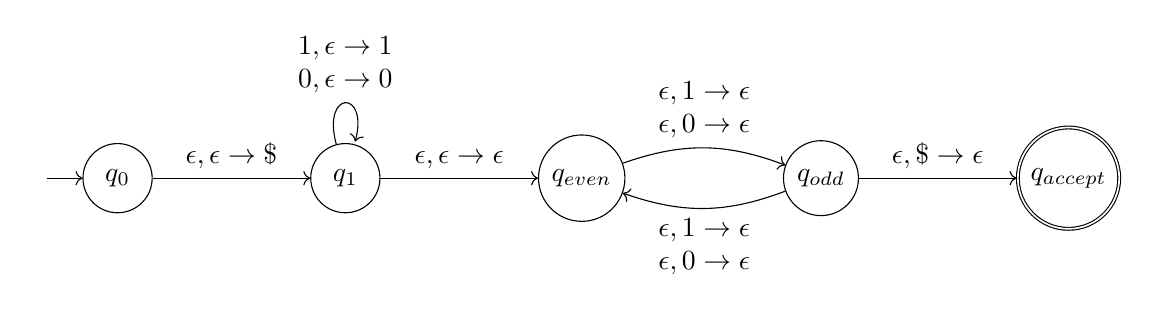
\begin{tikzpicture}
                   \node[state,initial] (q_0)   {$q_0$};
                   \node[state] (q_1) [right=2cm of q_0] {$q_1$};
                   \node[state] (q_2) [right=2cm of q_1] {$q_{even}$};
                   \node[state] (q_3) [right=2cm of q_2] {$q_{odd}$};
                   \node[state,accepting] (q_4) [right=2cm of q_3] {$q_{accept}$};
                    \path[->]
                    (q_0) edge [above] node {$\epsilon,\epsilon\rightarrow\$$} (q_1)
                    (q_1) edge [above] node {$\epsilon,\epsilon\rightarrow\epsilon$} (q_2)
                          edge [loop above, align=left] node {$1,\epsilon\rightarrow1$ \\ $0,\epsilon\rightarrow0$} (q_2)
                    (q_2) edge [bend left=20, above, align=left] node {$\epsilon,1\rightarrow\epsilon$ \\ $\epsilon,0\rightarrow\epsilon$} (q_3)
                    (q_3) edge [above] node {$\epsilon,\$\rightarrow\epsilon$} (q_4)
                          edge [bend left=20, below, align=left] node {$\epsilon,1\rightarrow\epsilon$ \\ $\epsilon,0\rightarrow\epsilon$} (q_2)
                    ;
                \end{tikzpicture}

                The idea here is we begin by placeing $\$$ on the stack.
                We then loop through the entire string in state $q_1$ and place each symbol in the stack.
                From this state, notice the only transitions are $\epsilon,x\rightarrow\epsilon$ where $x \in \Sigma_{\epsilon}$.
                This means we must have read all input here in $q_1$.
                Otherwise we the PDA will not have read all the input, and thus would fail.
                This also means we only care about the contents of the stack.

                We loop back and forth between $q_{even}$ and $q_{odd}$ after each element $x \in \Sigma$ is popped off the stack.
                This continues until the stack only contains $\$$.
                At this point, if we are in $q_{odd}$, this means we have popped an odd number of symbols off the stack, thus the string contained an odd number of symbols.

                As a note, it seems it would be relatively simple to build this logic as a normal NFA, without the use of a stack.
            \item
                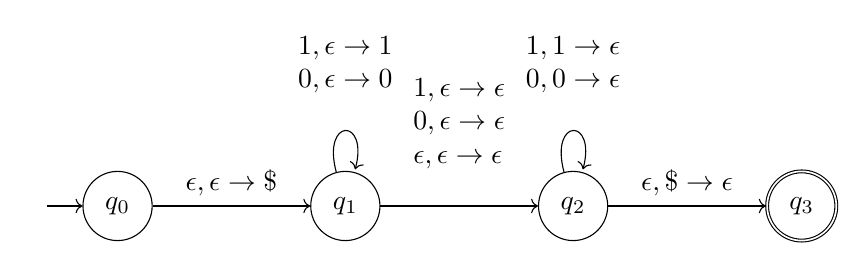
\begin{tikzpicture}
                   \node[state,initial] (q_0)   {$q_0$};
                   \node[state] (q_1) [right=2cm of q_0] {$q_1$};
                   \node[state] (q_2) [right=2cm of q_1] {$q_2$};
                   \node[state,accepting] (q_3) [right=2cm of q_2] {$q_3$};
                    \path[->]
                    (q_0) edge [above] node {$\epsilon,\epsilon\rightarrow\$$} (q_1)
                    (q_1) edge [above, align=left] node {
                          	$1,\epsilon\rightarrow\epsilon$ \\
                            $0,\epsilon\rightarrow\epsilon$ \\
                          	$\epsilon,\epsilon\rightarrow\epsilon$ \\
                          } (q_2)
                          edge [loop above, align=left] node {
                          	$1,\epsilon\rightarrow1$ \\
                            $0,\epsilon\rightarrow0$ \\
                          } (q_1)
                    (q_2) edge [above] node {$\epsilon,\$\rightarrow\epsilon$} (q_3)
                    	  edge [loop above, align=left] node {
                          	$1,1\rightarrow\epsilon$ \\
                            $0,0\rightarrow\epsilon$ \\
                          } (q_3)
                    ;
                \end{tikzpicture}

                Begin by adding $\$$ to the stack.
                Then the PDA reads some number of symbols onto the stack on $q_1$.
                The transition from $q_1$ to $q_2$ has a few options.
                We begin by observing $\epsilon,\epsilon\rightarrow\epsilon$.

                After this transition, we match each following symbol of the string to what has already been placed onto the stack.
                This matches palindromes because the stack is last in first out.

                Notice however, this only matches palindromes that are an even number of characters long.
                Odd length palindromes would have the center symbol placed on the stack, but would not match with the symbols on the right hand side.

                The other options in the transition from $q_1$ to $q_2$ allows a single symbol to be read and removed.
                The symbol does not effect the stack at all.
                This allows odd length palindromes.
            \item
                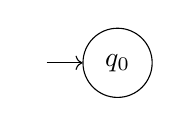
\begin{tikzpicture}
                   \node[state,initial] (q_0)   {$q_0$};
                \end{tikzpicture}

                There don't need to be any transitions, nor any accept states because nothing should ever be accepted.
        \end{enumerate}
    \item % 5
         $\Sigma: \set{2, +, \times, \left(, \right)}$ \\
                $\Gamma: \Sigma \cup \set{E, T, F}$

                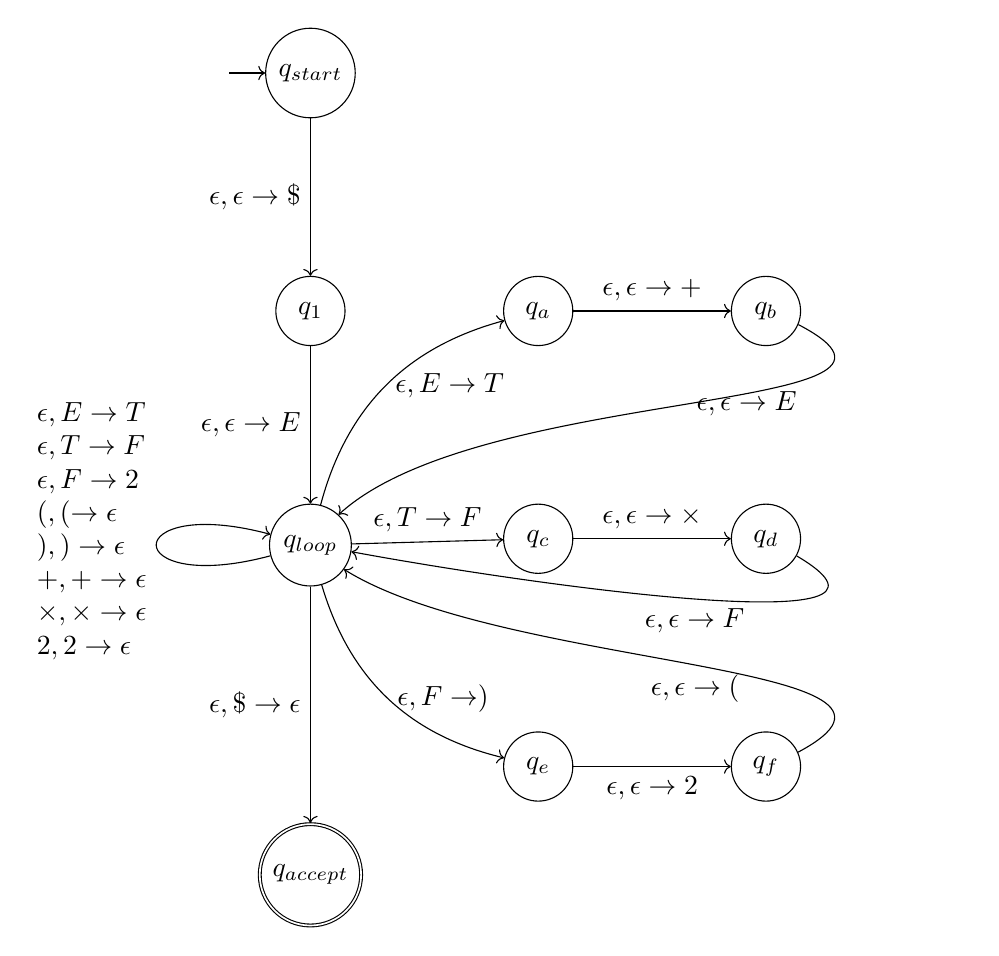
\begin{tikzpicture}
                      \node[state,initial] (q_0)   {$q_{start}$};
                      \node[state] (q_1) [below=2cm of q_0] {$q_1$};
                      \node[state] (q_loop) [below=2cm of q_1] {$q_{loop}$};
                      \node[state,accepting] (q_accept) [below=3cm of q_loop] {$q_{accept}$};
                      \node[state] (q_a) [right =2cm of q_1] {$q_a$};
                      \node[state] (q_b) [right=2cm of q_a] {$q_b$};
                      \node[state] (q_c) [below=2cm of q_a] {$q_c$};
                      \node[state] (q_d) [right=2cm of q_c] {$q_d$};
                      \node[state] (q_e) [below=2cm of q_c] {$q_e$};
                      \node[state] (q_f) [right=2cm of q_e] {$q_f$};
                      \path[->]
                            (q_0) edge [left] node {$\epsilon,\epsilon\rightarrow\$$} (q_1)
                            (q_1) edge [left] node {$\epsilon,\epsilon\rightarrow E$} (q_loop)
                            (q_loop) edge [left] node {$\epsilon,\$\rightarrow\epsilon$} (q_accept)
                            (q_loop) edge [bend left=30, right] node {$\epsilon,E \rightarrow T$} (q_a)
                                     edge [above] node {$\epsilon,T \rightarrow F$} (q_c)
                                     edge [bend right=30, right] node {$\epsilon,F \rightarrow )$} (q_e)
                                     edge [loop left, align=left, distance=2cm] node {
                                        $\epsilon, E \rightarrow T$ \\
                                        $\epsilon, T \rightarrow F$ \\
                                        $\epsilon, F \rightarrow 2$ \\
                                        $( , ( \rightarrow\epsilon$ \\
                                        $) ,) \rightarrow\epsilon$ \\
                                        $+,+ \rightarrow\epsilon$ \\
                                        $\times,\times \rightarrow\epsilon$ \\
                                        $2,2 \rightarrow\epsilon$ \\
                                     } (q_loop)
                             (q_a) edge [above] node {$\epsilon,\epsilon\rightarrow +$} (q_b)
                             (q_b) edge [bend right=230, in=200, right] node {$\epsilon,\epsilon\rightarrow E$} (q_loop)
                             (q_c) edge [above] node {$\epsilon,\epsilon\rightarrow \times$} (q_d)
                             (q_d) edge [bend left=150, in=170, below] node {$\epsilon,\epsilon\rightarrow F$} (q_loop)
                             (q_e) edge [below] node {$\epsilon,\epsilon\rightarrow 2$} (q_f)
                             (q_f) edge [bend left=230, in=170, below] node {$\epsilon,\epsilon \rightarrow ($} (q_loop)
                        ;
                \end{tikzpicture}
\end{enumerate}

\end{document}
